\documentclass[10pt, aspectratio = 169]{beamer} % All teh graphics are calibrated for this size 

% Theme choice
\usetheme{simpleMIA}
\usecolortheme{default}

% Import packages
\usepackage{float}
\usepackage{algorithm}
\usepackage{algpseudocode}

% Title page information 
\title{Neural Nets are crazy cool}
\subtitle{Some fancy subtitle \\ in 2 lines maybe} % Optional
\author{Jean Dupont and Jeannet Dupont}
\shortname{J. Dupont \& J. Dupont} % Optional
\supervisors[Supervised by]{\textbf{Prof.1} and \textbf{Prof.2}} % Optional
\date{\today} % Optional

% Declare all the logos
\setLogo{assets/logo_mia_no_text.png}
\setTitleLogoLeft{assets/MIA_ekinocs_logo.png} % Change this according to your team {ekinocs, solstis}
\setTitleExtraLogo{assets/logo_inrae.png} % Optional for other affiliations
\setTitleExtraLogoTwo{assets/logo_apt.png} % Optional for other affiliations


\begin{document}

% Title slide
\begin{frame}
    \titlepage
\end{frame}

% Outline slide
\begin{frame}
    \frametitle{Outline}
    \tableofcontents
\end{frame}

% New slide
\section{An artificial neuron !}
\begin{frame}
    \frametitle{The McCulloch-Pitts Model}
    \setbeamercovered{transparent}
    \begin{columns}
    	\column{0.5\textwidth}
	    	\begin{itemize}
	    	\pause
	    	\item This is the first point
		    	\begin{itemize}
		    		\item This is a second hierarchy point
		    	\end{itemize}
		    \pause
	    	\item Here's the second point
	    	\pause
	    	\item And a third point
	    	\end{itemize}
	    	\pause
	    	\begin{block}{The equation of a Neural Network}
	    		The equation gouverning neuron $k$ is :
	    		\[\text{Output}_k = \varphi(\sum_{1}^{m} x_i w_{ki} + \text{Bias})\]
	    	\end{block}
    	\column{0.5\textwidth}
    	\centering 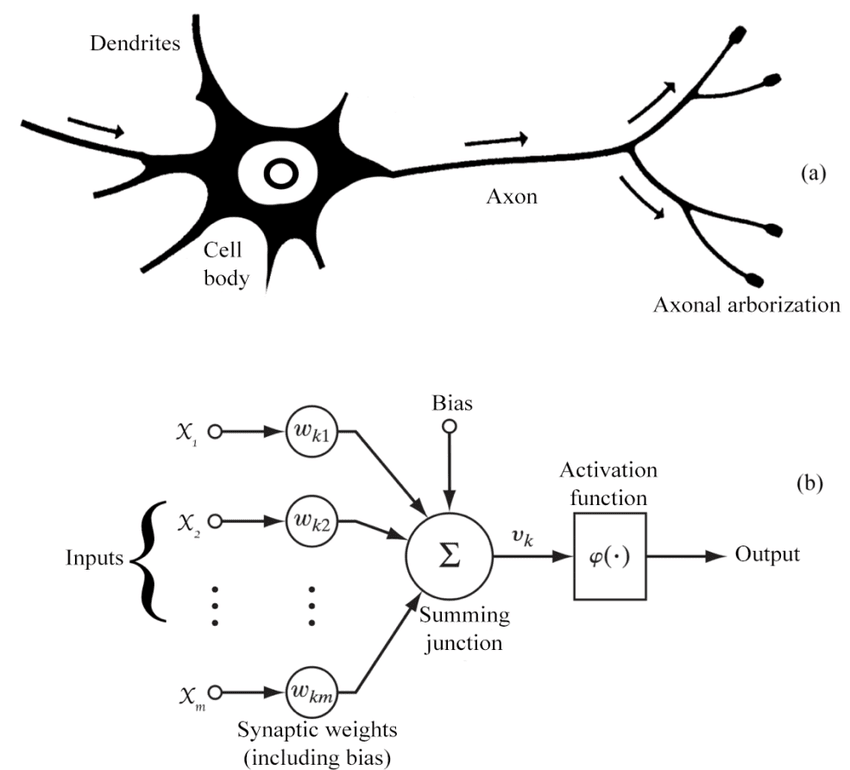
\includegraphics[width=\textwidth]{images/artificial_neuron.png}
    \end{columns}
\end{frame}

% New slide
\begin{frame}
	\frametitle{Backpropagation}
	\begin{algorithm}[H]
		\caption{Hyper symple Backprop}
		\begin{algorithmic}
			\small
			\State For a sample $(x_n ,y^*_n)$, propagate the input $x_n$ through the network to compute the outputs $(v_{i_1}, \ldots, v_{i_{|V|}})$ (in topological order).
			\vspace{0.2cm}
			\State Compute the loss $\mathcal{L}_n := \mathcal{L}(v_{i_{|V|}}, y_n^*)$ and its gradient.
			\begin{align}
				\frac{\partial \mathcal{L}_n}{\partial v_{i_{|V|}}}.
			\end{align}
			\For{$j \in |V|,\ldots,1$}
				\begin{align}
					\frac{\partial \mathcal{L}_n}{\partial w_j} =
					\frac{\partial \mathcal{L}_n}{\partial v_{i_{|V|}}} \prod_{k = j + 1}^{|V|} \frac{\partial v_{i_k}}{\partial v_{i_{k - 1}}}
					\frac{\partial v_{i_j}}{\partial w_j}.
				\end{align}
				where $w_j$ refers to the weights in node $i_j$.
			\EndFor			
		\end{algorithmic}
	\end{algorithm}
\end{frame}

% Content slide 3
\section{Other aspects of the template}
\begin{frame}
    \frametitle{Blocks!}
    \begin{block}{This is a Block}
        This is the primary colour
    \end{block}
    \pause
    \begin{exampleblock}{This is an Example Block}
        This is derived from the primary colour
    \end{exampleblock}
    \pause
    \begin{alertblock}{This is an Alert Block}
        This is also derived from the primary colour
    \end{alertblock}
\end{frame}


\end{document}